\documentclass{article}
\usepackage{multirow}
\usepackage{Sweave}
\begin{document}
\Sconcordance{concordance:draft1.tex:draft1.Rnw:%
1 2 1 1 0 4 1 1 8 59 1 1 11 13 1 1 8 17 1 1 8 299 1}





\section*{Abstract}

Community-driven online question and answer forums (CQA) house an expansive amount of crowd-sourced knowledge in the form of thousands of questions and answers posted everyday. Forums can cover a broad range of topics, like \textit{Yahoo! Answers}, or can be focused on a specific topic, like computer programming-focused \textit{Stack Overflow}. An example of the latter is iFixit's \textit{Answers} forum. The \textit{Answers} forum features user-asked questions related specifically to device repair, which are answered by both repair experts and everyday users, furthering iFixit's mission to enable individuals to repair their own devices. As such, it is important that questions receive timely answers. This paper presents a survival analysis on the time until a question receives its first answer. We developed a Cox proportional hazards model to predict the failure probability of a question, or the probability that a question receives an answer before a certain time. Though we identified signifcant predictors, the predictive accuracy was low ($R^2 = 0.15$). Our findings indicate that the most important predictors were the device category of the question (questions pertaining to Apple products received answers faster than others (HR = 2.56, 95\% CI = (2.31, 2.82))) and factors related to the question's title (e.g., whether or not it was phrased as a question (HR = 1.31, 95\% CI = (1.22, 1.41))). Future studies could investigate if the factors identified as signifcant in our study can be generalized to other CQAs. 


\section*{Introduction}

Community-driven online question and answer forums (CQA) are becoming widely used sources of information. These online platforms allow for anyone to ask or answer a question, regardless of their background or expertise level. Forums can receive around 40 million visits every month.
    
The CQA analyzed in this paper is iFixit's \textit{Answers} forum. Founded in 2003, iFixit's mission is to enable people to repair their broken devices, effectively saving them money and reducing electronic waste. The company provides over 30,000 free online repair guides and sells the specialized tools and parts needed for such repairs.
    
As not all possible repairs are covered in the published repair guides, and users may have questions related to those guides, iFixit's \textit{Answers} forum is another important resource. This platform features questions pertaining to over 9,000 devices with over 100,000 solutions. Questions range from broken devices like jammed zippers to shattered iPhone screens. As many rely on this forum for help with repairs, it is important that users receive timely answers. Fast response times will enhance user engagement and generate more web traffic, which is valuable to the reputation and longevity of the \textit{Answers} forum. Analysis of answer times can reveal factors that affect how quickly questions are answered, which can lead to suggestions for how users can ask better questions to minimize answer times, and for how the forum design can be improved. 
However, analysis and prediction of answer \textit{times} on CQAs have not been thoroughly investigated. As the majority of existing research focuses on assessing and predicting question and answer quality, there is need for further analysis of response times in these forums. This paper presents a survival analysis on the time until a question is answered on iFixit's \textit{Answers} forum, in order to determine factors significantly related to answer time and to predict the ``survival'' probability of a question.


\section*{Related Work}
  
In regards to investigation of forum response times, \citep{Bhat2014} developed a classification model to analyze response times of questions posted on \textit{Stack Overflow}, and found that tag-based features like the number of tags included or the number of subscribers a certain tag has, were the best predictors of answer time. 

\citep{Mamykina2011} found that the swift answer times of \textit{Stack Overflow's} community is a result of the reputation system and the strict emphasis on factual and informative questions and answers, rather than discussion-based. 

\citep{Asaduzzaman2013} analyzed unanswered questions on \textit{Stack Overflow} to determine common characteristics and found that questions that went unanswered shared certain characteristics in that they were too short and vague, or utilized the tagging system incorrectly. 



\section*{Materials}

good question ex: id 408124, 406786 (answered)
bad question ex: id 410310, 405882 (unanswered) 

The data analyzed contained 8,025 questions posted from April 8, 2017 (10:14 PM) to July 7, 2017 (9:28 PM) (the date the data was downloaded). Variables in the data included: device name and category, title, text, tags, whether or not the user was a member of iFixit's site for less than one day before the question was posted, date the question was posted, date the first answer was received. Variables derived: 

Categorical Variables: 

\begin{itemize}
  \item Device category the question pertains to. Categories include: Apple Products, Android\/Other Phone, PC, Tablet, Electronics, Camera, Vehicle, Game Console, Home, Other.
  \item Whether or not the question's title contains at least one word that is considered ``frequently used'' among answered questions. See appendix for a complete list of these terms. 
  \item Whether or not the question's title contains at least one word that is considered ``frequently used'' among unanswered question. See appendix for a complete list of these terms. 
  \item Whether or not the question's title ends in a question mark.
  \item Whether or not the question's text contains any end punctuation marks (. ? !). 
  \item Whether or not the question's text is in all lower case. 
  \item Whether or not the user edited or added information to the question's text sometime after posting it.
  \item Whether or not the user made an effort to solve the problem on their own, prior to asking the question.
  \item The day of the week the question was posted. 
\end{itemize}

Numeric Variables:

\begin{itemize}
  \item The average tag ``score'' for all of a question's tags. A tag score is defined as the proportion of times a tag appears in all of the data. Questions without tags were assigned an average tag score of 0. 
  \item The average number of characters in each question's tags. 
  \item The number of characters in the question's text. 
  \item The number of characters in the user-defined device name. 
  \item The ratio of the number of line breaks to the number of characters in the question's text.
\end{itemize}



\section*{Methods}



Questions analyzed were restricted to those posted in English. The time until event variable used in survival analysis was defined as the time since posting until a question received its first answer. For questions that did not receive an answer by the download date, time until event values were defined as the time since posting to the time the data was downloaded. These questions were considered right-censored, meaning that exact answer times for these questions are greater than the times in the data (questions can still receive answers after the download date). 

Survival was defined as the event that a question did not receive an answer beyond a certain time, t. Estimates of survival probability were generated with the Kaplan-Meier method, which adjusts to the presence of right-censored, or unanswered questions (cite). From these estimates, survival curves were constructed to examine the survival experience of questions. Mean, median and other percentiles of survival times were also generated. 

As the probability distribution for answer times was unknown, a nonparametric Cox proportional hazards model was developed to predict survival probability (Cox models are not based on an assumption of the shape of the underlying probability distribution (cite)). To build the model, five-fold cross-validation was used. The full data was split into five training and five test sets. Each training set contained 6208 questions, and each test set contained 1552 questions. Univariate analysis, performed on one of the training sets, was used to identify variables to potentially include in the final Cox proportional hazards model. Distributions of continuous variables constructed on one of the training sets, were assessed and transformations were applied. Each categorical and continuous predictor, both with and without transformations, were entered into separate Cox models and strength of association with answer times were assessed. Those with partial likelihood ratio test p-values of less than 0.01 were included in the full model for cross-validation.

In each fold of cross-validation, the full model, with variables found to be signficant in univariate analysis, was built on one of the training sets and used to generate predicted hazard ratios on the corresponding test sets. To assess prediction performance, the predicted hazard ratios were entered into separate Cox models as the single quantitative predictor with answer times as the survival time. The resulting estimated hazard ratio, R-square statistic, partial likelihood ratio and p-value were assessed as indicators of the full model's performance \citep{Chen}. Signficant statistics would indicate high predictive accuracy. Concordance statistics and Somers' Dxy were also assessed to measure the model's predictive discrimination. Concordance is defined as the probability that for any two randomly chosen questions, the question with the shorter survival time also has the higher predicted hazard. Concordance statistics close to 1 indicate high discriminative ability, while statistics close to 0.5 indicate discordance, or random predictions. Somers' Dxy is the difference between the model's concordance statistic and discordance, 0.5 \citep{Harrell2015}. These metrics were computed for each training and test set. The averages of metrics across test sets were evaluated. The final model was selected based on AIC statistics and the signficance of prediction metrics, as well as how consistent those metrics were across training and test sets. The final model was then fit to the full data and the same metrics were computed and compared. 

Plots of Martingale residuals, the differences between observed number of answers received by each question and the expected number of answers expererienced by each question under the model, were evaluated to assess functional form of each continuous predictor. Deviance residuals, which are transformed Martingale residuals with a mean of 0 and an approximately normal distribution, were assessed to identify questions poorly predicted by the model. Score residuals, a measure of the approximate change in parameter estimates that would occur if a question were removed from the sample, were assessed to check for questions that highly effect parameter estimates. 

Restricted cubic splines were applied to all continuous predictors \citep{Harrell2015}. Splines of five knots were initially fit to each. A higher number of knots were assigned to predictors hypothesized to be more signficant, those with lower model p-values. The optimal number of knots for each predictor was determined based on the model AIC statistic. 

Correlations between scaled Schoenfeld residuals, the differences between observed and expected predictor values for questions that received answers, and a function of time, were examined to assess the proportional hazards assumption that underlies a Cox model. Proportional hazards assumes that the effect of predictors on hazard does not depend on time. Significant correlations indicate that a predictor has violated this assumption. 


\section*{Results}


\begin{figure}[h!]
  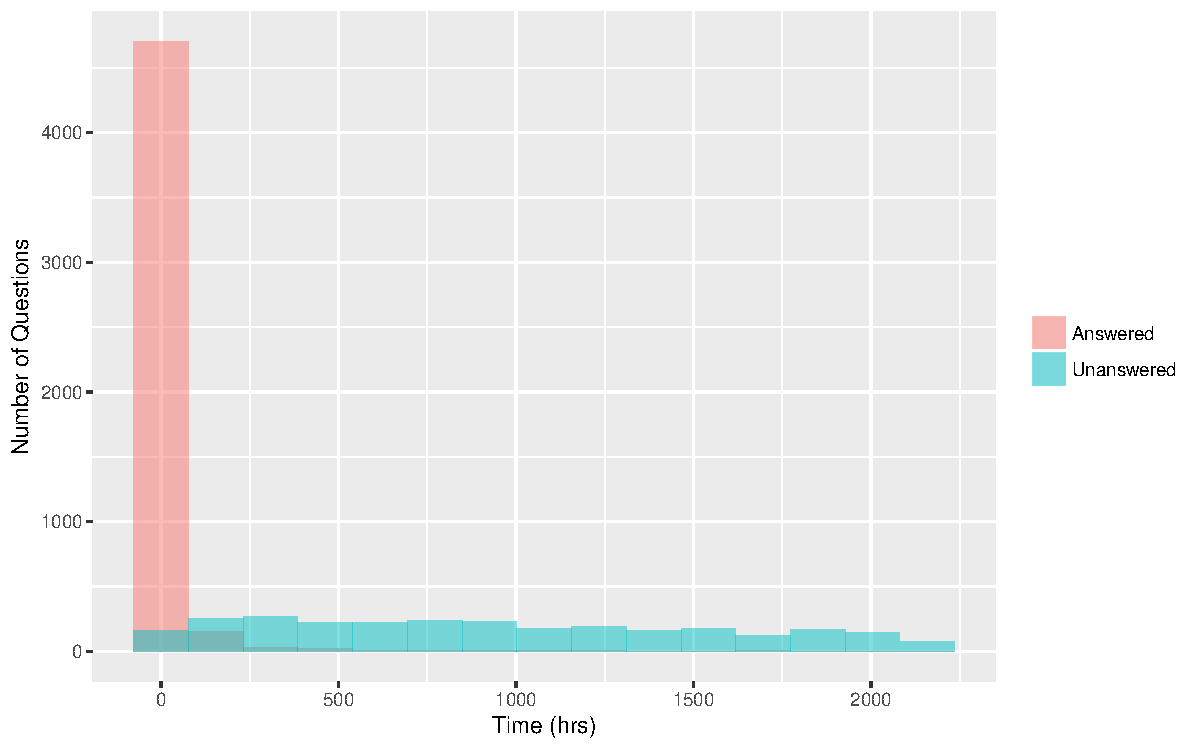
\includegraphics[scale=1]{times_dist.pdf}
  \caption{Distribution of answer times}
  \label{fig:answertimes}
\end{figure}

\begin{figure}[h!]
  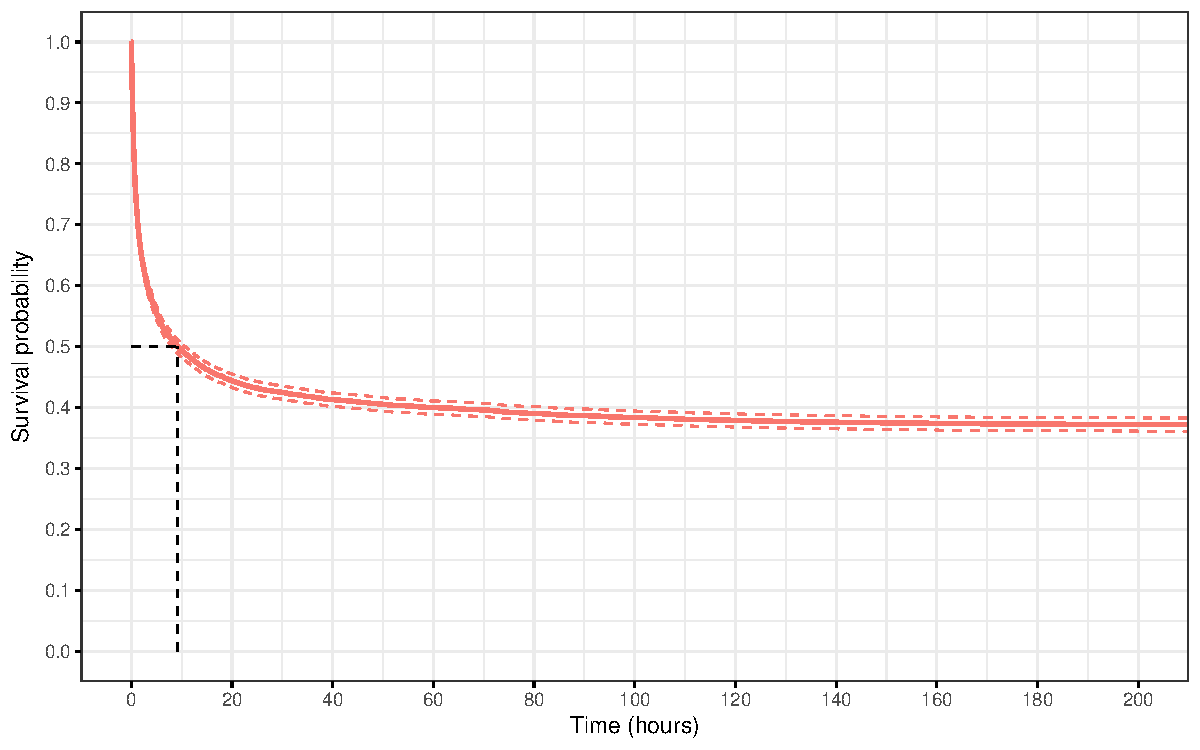
\includegraphics[scale=1]{kmcurve.pdf}
  \caption{Kaplan-Meier curve for all questions}
  \label{fig:kmcurve}
\end{figure}

  Of 8,025 questions in the full data set, 7760 were in English (97\% of the full data). Of those questions, 4951 (63.8}\%) received an answer by the download date. The shortest answer time was 0.5 hours. The longest was 2159.02 hours (89.96 days). Figure ~\ref{fig:answertimes} shows the distribution of answer times for all questions, grouped by whether or not the question received an answer. 



\begin{table}[ht]
\centering
\begin{tabular}{rlr}
  \hline
 Percent\\ Answered & Time (hrs) \\ 
  \hline
  25 & 0.88 \\ 
  50 & 9.16 \\ 
  55 & 18.38 \\ 
  58 & 33.71 \\ 
  60 & 59.47 \\ 
  64 & 683.19 \\ 
   \hline
\end{tabular}
\caption{Table of Kaplan-Meier estimated quantiles of survival time}
\label{table:quantiles}
\end{table}

  Figure  ~\ref{fig:kmcurve} shows the Kaplan-Meier curve of survival probability for all questions in the data. The curve indicates that around 150 hours after a question has been posted, survival probability coasts at around 0.35 and never reaches 0, indicating that if a question does not receive an answer within the first 100 hours, the likelihood of it receiving an answer in the future is low. The Kaplan-Meier estimated mean survival time, or the average time until a question received its first answer was 775.75 hours, or 32.32 days. The median survival time, the time at which 50\% of the questions in the data received an answer, was 9.16 hours. Table \ref{table:quantiles} provides additional percentiles of survival time.

\begin{table}[ht]
\centering
\caption{Univariate analysis results for quantitative predictors, ordered by increasing p-values} 
\begin{tabular}{|p{12cm}|p{2cm}|}
  \hline
  Predictor & p-value \\ 
  \hline \hline
  Log transformation of the number of characters in a question's text* & 0.00 \\ 
  \hline
  Square root transformation of the number of characters in a question's text* & 0.00 \\ 
  \hline
  Number of characters in a question's text (untransformed) & 0.00 \\
  \hline
  Square root transformation of the ratio of the number of line breaks to the number of characters in a question's text* & 0.00 \\ 
  \hline
  Square root transformation of the average frequency ``score'' of a question's tags* & 0.00 \\ 
  \hline
  Average frequency ``score'' of a question's tags (untransformed) & 0.00 \\ 
  \hline
  Ratio of the number of line breaks to the number of characters in a question's text (untransformed) & 0.00 \\ 
  \hline
  Square root transformation of the number of characters in the user-defined device title* & 0.00 \\ 
  \hline
  Square root transformation of the average number of characters in a question's tags* & 0.00 \\ 
  \hline
  Number of characters in the user-defined device title (untransformed) & 0.01 \\ 
  \hline
  Average number of characters in a question's tags (untransformed) & 0.03 \\ 
   \hline
\end{tabular}
\label{table:qresults}
\end{table}

\begin{table}[ht]
\centering
\caption{Univariate analysis results for categorical predictors, ordered by increasing p-values} 
\begin{tabular}{|p{12cm}|p{2cm}|}
  \hline
 Predictor & p-value \\ 
  \hline \hline
  Device category & 0.00 \\
  \hline
  Whether or not the user had been a member for less than one day before the question was posted & 0.00 \\ 
  \hline
  Whether or not the question's title ended in a questionmark & 0.00 \\ 
  \hline
  Whether or not the question's text contained at least one end punctuation mark & 0.00 \\ 
  \hline
  Day of the week the question was posted & 0.00 \\ 
  \hline
  Whether or not the question's text is in all lower case & 0.00 \\ 
  \hline
  Whether or not the user made an effort to solve the problem on their own, prior to asking the question & 0.00 \\ 
  \hline
  Whether or not the user edited or added information to the question's text sometime after posting it & 0.00 \\
  \hline
  Whether or not the question's title contains terms considered to be frequently used among unanswered questions & 0.00 \\ 
  \hline
  Whether or not the question's title contains terms considered to be frequently used among answered questions & 0.00 \\ 
   \hline
\end{tabular}
\label{table:cresults}
\end{table}

Results of univariate analyis for transformed and untransformed quantitative predictors, and categorical predictors, are are shown in Table \ref{table:qresults} and Table \ref{table:cresults}, respectively. All categorical predictors were entered into the full model. Restricted cubic splines were fit to all * quantitative variables.

\begin{table}[ht]
\centering
\caption{Determining the optimal k number of splines for each predictor} 
\begin{tabular}{| p{5cm} | l | l | l |}
  \hline
  Predictor & K & p-value & AIC \\ 
  \hline
  \multirow{ 4 }{ 5cm }{Log transformation of the number of characters in a question's text} 
  & 0 & 0.00 & 65862.83 \\ 
  & 5* & 0.00 & 65862.02 \\ 
  & 4 & 0.00 & 65863.35 \\ 
  & 3 & 0.00 & 65862.08 \\ 
  \hline
  \multirow{ 4 }{ 5 cm }{Square root transformation of the ratio of the number of line breaks to the number of characters in a question's text}
  & 0 & 0.00 & 65890.28 \\ 
  & 5 & 0.00 & 65884.70 \\ 
  & 4 & 0.00 & 65882.98 \\ 
  & 3* & 0.00 & 65881.93 \\ 
  \hline
  \multirow{ 4 }{ 5 cm }{Square root transformation of the average frequency ``score'' of a question's tags}
  & 0* & 0.00 & 65890.75 \\ 
  & 5 & 0.00 & 65891.69 \\ 
  & 4 & 0.00 & 65891.75 \\ 
  & 3 & 0.00 & 65892.35 \\ 
  \hline
  \multirow{ 4 }{ 5 cm }{Square root transformation of the number of characters in the user-defined device title}
  & 0 & 0.00 & 65922.76 \\ 
  & 5* & 0.00 & 65853.56 \\ 
  & 4 & 0.00 & 65882.07 \\ 
  & 3 & 0.00 & 65881.39 \\ 
  \hline
  \multirow{ 4 }{ 5 cm }{Square root transformation of the average number of characters in a question's tags}
  & 0 & 0.00 & 65923.26 \\ 
  & 5 & 0.00 & 65912.11 \\ 
  & 4* & 0.00 & 65910.10 \\ 
  & 3 & 0.00 & 65912.38 \\ 
   \hline
\end{tabular}
\label{table:splines}
\end{table}

Table \ref{table:splines} shows the results of determining the optimal number of knots for each quantitative predictor. Knots marked * were included in the final model for cross-validation. 

\begin{table}[ht]
\centering
\caption{Average performance metrics for training and test sets} 
\begin{tabular}{rrrrrrrr}
  \hline
 & HR & LR & pval & R2 & AIC & Dxy & Concordance \\ 
  \hline
  Training Set & 2.00 & 959.49 & 0.00 & 0.14 & 64729.80 & 0.27 & 0.64 \\ 
  Test Set & 1.96 & 225.44 & 0.00 & 0.14 & 13453.18 & 0.26 & 0.63 \\ 
   \hline
\end{tabular}
\label{table:cv}
\end{table}

Average performance metrics for test and training sets, found in Table \ref{table:cv}, were considerably low. However, metrics did not change substantially from training to test sets, indicating that the model does not overfit. The final model, with all variables described above including splines, was fit to the full data.

\begin{table}[ht]
\centering
\caption{P-values for final model fit to the full data} 
\begin{tabular}{|p{12cm}|p{1cm}|}
  \hline
Predictor & p \\ 
  \hline \hline
Device Category & 0.00 \\ 
  \hline
Whether or not the user had been a member for less than one day before the question was posted & 0.00 \\ 
  \hline
Whether or not the question's title contains terms considered to be frequently used among unanswered questions & 0.00 \\
  \hline
Whether or not the question's title contains terms considered to be frequently used among answered questions & 0.22 \\ 
  \hline
Whether or not the question's title ended in a questionmark & 0.00 \\ 
  \hline
Whether or not the question's text contained at least one end punctuation mark & 0.53 \\ 
  \hline
Whether or not the question's text is in all lower case & 0.01 \\ 
  \hline
Whether or not the user edited or added information to the question's text sometime after posting it & 0.00 \\ 
  \hline
Whether or not the user made an effort to solve the problem on their own, prior to asking the question & 0.01 \\ 
  \hline
Day of the week the question was posted & 0.00 \\ 
  \hline
Square root transformation of the average frequency ``score'' of a question's tags & 0.00 \\ 
  \hline
Square root transformation of the average number of characters in a question's tags & 0.05 \\ 
Nonlinear & 0.08 \\ 
  \hline
Square root transformation of the number of characters in a question's text & 0.43 \\ 
Nonlinear & 0.46 \\ 
  \hline
Square root transformation of the number of characters in the user-defined device title & 0.28 \\ 
Nonlinear & 0.42 \\ 
  \hline
Square root transformation of the ratio of the number of line breaks to the number of characters in a question's text & 0.36 \\ 
Nonlinear & 0.62 \\ 
   \hline
\end{tabular}
\label{table:pvalues}
\end{table}

\begin{table}[ht]
\centering
\begin{tabular}{rlr}
  \hline
 & variable & coefficients \\ 
  \hline
1 & new\_category=Apple Product & 0.93 \\ 
  2 & new\_category=Camera & -0.26 \\ 
  3 & new\_category=Electronics & -0.08 \\ 
  4 & new\_category=Game Console & 0.21 \\ 
  5 & new\_category=Home & 0.39 \\ 
  6 & new\_category=Other & -0.11 \\ 
  7 & new\_category=PC & 0.43 \\ 
  8 & new\_category=Tablet & -0.15 \\ 
  9 & new\_category=Vehicle & 0.38 \\ 
  10 & new\_user=1 & -0.10 \\ 
  11 & contain\_unanswered & -0.27 \\ 
  12 & contain\_answered & 0.05 \\ 
  13 & title\_questionmark & 0.25 \\ 
  14 & text\_contain\_punct & 0.03 \\ 
  15 & text\_all\_lower & -0.18 \\ 
  16 & update & 0.28 \\ 
  17 & prior\_effort & -0.09 \\ 
  18 & weekday=Monday & 0.01 \\ 
  19 & weekday=Saturday & -0.07 \\ 
  20 & weekday=Sunday & -0.11 \\ 
  21 & weekday=Thursday & 0.03 \\ 
  22 & weekday=Tuesday & 0.09 \\ 
  23 & weekday=Wednesday & 0.10 \\ 
  24 & avg\_tag\_score & 2.23 \\ 
  25 & avg\_tag\_length & -0.08 \\ 
  26 & avg\_tag\_length' & 0.58 \\ 
  27 & avg\_tag\_length'' & -1.52 \\ 
  28 & text\_length & -0.08 \\ 
  29 & text\_length' & -0.36 \\ 
  30 & text\_length'' & 2.39 \\ 
  31 & text\_length''' & -3.69 \\ 
  32 & device\_length & -0.07 \\ 
  33 & device\_length' & 0.18 \\ 
  34 & device\_length'' & -0.27 \\ 
  35 & device\_length''' & 0.21 \\ 
  36 & newline\_ratio & 0.12 \\ 
  37 & newline\_ratio' & 0.36 \\ 
   \hline
\end{tabular}
\caption{Coefficients for predictors in the final model} 
\label{table:coefficients}
\end{table}

Score and deviance residuals of the final model identified outliers and highly influential questions. However, because refitting the model without those questions resulted in worse predictive accuracy, all questions were left in the data. Assessing the proportional hazards assumption indicated that several predictors were in violation. P-values for the correlation between predictors schoenfeld residuals and time are shown in table e. But as stratifying on this predictor substantially decreased predictive accuracy, the variable was left as is. Statistics and parameter coefficients of the final model are in table c. Metrics for the final model's performance on the full data, though considerably low, are not different from the metrics computed in cross-validation. 

\section*{Discussion}

(Discuss importance of findings, not repeat them. A combined results + discussion section is often appropriate) 
The data we analyzed for this model presented some limitations. Currently, askers have a considerable amount of freedom in the way they ask a question. As a result many incorrectly specify various input fields. For example, a question about a faulty Android tablet screen included as a tag ``someone sat on it :(''. Generally, tags are not more than a couple key words that describe the topic of the question. Many users on this forum included lengthy and somewhat ambiguous tags in their question. Another issue was the incorrect naming of the device the user's question was about. A user asking a question about their Turtle Beach Ear Force X device included as the name of their device "Turtle Beach Ear Force Xmy grandson chewed through the wire while we was playing it's brand-new is there anyway I can have it fixedO One". The inconsistencies in this data made it somewhat difficult to analyze, and possibly contributed to the model's low predictive accuracy. 

\section*{Conclusion}

This study developed a Cox regression model to predict the probability that a question posted on iFixit's \textit{Answers} forum receives an answer before a certain time. Predictors found to be signficant in the model included: device category, whether or not the question contained words considered to be ``frequently-used'' among unanswered questions, whether or not the title ends in a questionmark, whether or not the user updated the question's text after the initial posting, whether or not the user indicated that he or she made an effort prior to answer their question prior to posting it (how should I write out that different knots of the splines were signficant). While overall the model was signficant, its predictive performance was considerably low. 

\section*{Acknowledgement}

This research is supported by the Bill and Linda Frost fund. 

\section{Appendix} 

device

The original device categorization variable, as defined by iFixit, included: Apparel, Appliance, Camera, Car and Truck, Computer Hardware, Electronics, Game Console, Household, Mac, Media Player, PC, Phone, Skills, Tablet, Vehicle. This variable also contained a considerable amount of NAs (1954, or 25.2\% of all questions). NAs are a result of users asking questions for devices not already in the website's database, or from the user incorrectly defining the device. 


This category variable contained NAs (include how many), a result of the asker creating a question for a device not already on the website's data base. Questions that made the device clear were categorized accordingly. However there were a number of questions that did not explicitly declare the device their question pertained too. These questions were categorized as ``Other''. All Apple products (e.g., iPhones, iMacs, Apple watches) were given their own category. After pulling out iPhones from the original ``Phones'' category, the remaining phones were categorized as ``AndroidOther Phone''. Appliance and Household categories of the original variable were merged into ``Home''. ``Car and Truck'' were added to the ``Vehicle''. Lastly, any category that contained less than 2\% of the questions were categorized as ``Other''. All other categories remained the same as the original category. The final categories in the new categorization variable were Apple Product, Android/Other Phone, PC, Tablet, Electronics, Camera, Vehicle, Game Console, Home, and Other. 

contain answered and unanswered

  These variables were created based on the intuition that certain topics might be more popular, and even unpopular, among the answering community, and that questions concerning these topics might recieve an answer faster, or slower, than questions that don't. 
  
  To create these variables, the data was separated between answered and unanswered questions. Using text mining techniques, two lists were created-one for answered questions and another for unanswered questions--containing every word within the question's titles and the frequency or the number of time they occured among answered and unanswered questions. For ``frequently-used'' words in answered questions, that word would have to appear in more than 1\% of answered question's titles, and would have to appear in answered questions more than it appeared in unanswered questions. To determine the latter, a ratio of proportions was assessed. This ratio was calculated as the proportion of times a word occured among answered questions, to the proportion of times a word occured in unanswered questions. As an example, if ``cracked'' appeared in 2\% of answered questions and in 0.1\% of unanswered questions, it would be considered frequently used among answered questions as it occurs in more than 1\% of answered question's titles and occurs 20 times more in answered questions and in unanswered questions (ratio = 0.02/0.001 = 20). As for ``frequently-used'' words in unanswered questions, they must occur in 1\% or more of the question's titles and occur in more unanswered questions than unanswered questions (ratio < 1). Since there was some overlap between the words in each list and the device categories, every word that matched a device name was removed from the list. The resulting list for answered questions was 111 words, and 32 words in uanswered questions. Contain\_answered and contain\_unasnwered are logical variables, indicating true if a question's title contained at least one of the words in the frequently used words list for answered and unanswered questions, respectively. 
  
111 terms found to be ``frequently-used'' among answered questions (ordered from highest frequency): 
screen, turn, working, replacement, power, work, replace, charging, charge, button, touch, black, turning, broken, start, stuck, new, lcd, upgrade, problem, change, port, replaced, card, open, boot, replacing, remove, reset, back, drive, error, cable, ssd, cracked, hard, one, dropped, logic, lines, white, keeps, pro, dead, now, front, damage, switch, parts, glass, still, charger, issue, sim, turns, digitizer, just, mode, model, backlight, usb, stopped, logo, starting, know, unresponsive, password, factory, call, use, damaged, find, sensor, possible, fixed, side, galaxy, data, ipod, problems, issue, slow, system, connector, without, overheating, code, ram, air, microphone, please, red, much, plugged, getting, booting, left, way, buy, plus, time, loose, lock, coming, got, shuts, says, install, key, door, top

32 terms found to be ``frequently-used'' among unanswered questions (ordered from highest frequency):
sound, light, wifi, speaker, connect, picture, stay, noise, bluetooth, isnt, apps, going, rear, question, play, stop, service, take, hear, lights, showing, network, volume, come, keep, connection, flashing, shut, print, blue, buttons, edit
  
Text\_contain\_punct

A logical variable indicating true if the question’s text contains any end punctuation marks (. ? !). This variable was created to investigate if run-on sentences, or sentences with no end punctuation, take longer to receive an answer. 

Prior\_effort 

Logical variable indicating true if the asker used words that indicate prior effort or research was done before asking the question (e.g. ``tried'', ``attempted'', ``tested''). This variable was created based off of findings from \cite{Bhat2014}. 

Avg\_tag\_score

This variable was created to investigate the idea that some tags are more popular, or widely used than other, and that including such tags might increase the likelihood of that question recieving an answer. This variable is the average frequency, or proportion of times a question's tags appear in all of the data set. If a question has a higher average, than at least one of it's tags are frequently used. This variable was created based off of findings from \cite{Bhat2014}. 

Device\_length

The number of characters in the user-defined device variable. This variable was included to capture when a user incorrectly inputs the device name. For example, the device variable for question 390271 is, “Turtle Beach Ear Force Xmy grandson chewed through the wire while we was playing it's brand-new is there anyway I can have it fixedO One” and is 136 characters long. 11 questions in this data set also didn’t include any device. This variable was created based on the intuition that users who incorrectly define their devices make it harder for answerers to discern the topic of their question, and thus have longer answer times or might not recieve an answer.

Avg\_tag\_length

The average number of characters in each question's user-defined tags. If a question did not include a tag, this variable was set to 0. This variable, like the device-length variable, was created to capture when a user correctly or incorrectly used the tagging system. For example, question 390989 includes tag: “i need to repair the headset because i can not find the bluetoot” and is 64 characters long, while question 410254 includes tags "sound", "sound driver" and "speaker" and has an average tag length of 8 characters. It is hypothesized that users who use the tagging system correctly, as with the latter user, receive answers quicker than the former user. 

Newline\_ratio

This ratio of the number of newlines to the number of characters in the question's text. This variable was based on the intuition that question's that include newlines in the text are easier to read and thus have faster answer times. Questions with long text that also include newlines are generally easier to read than questions that don’t include any. 

\bibliographystyle{ECA_jasa}
\bibliography{questions}








\end{document}
